\documentclass[a4paper]{article}
\usepackage[spanish]{babel}  %babel es el paquete de idiomas y antes de eso va el o los idiomas que se reuqieren emplear
\usepackage[colorlinks=true, citecolor=blue, final]{hyperref}
\usepackage{url} % UTILIZA EL PAQUETE PARA QUE APAREZCA EL URL AUNQUE AUN NOSE SI DEBO ACTIVARLO TAMBIEN EN REFERENCIAS
\hypersetup{
    colorlinks=true,
    linkcolor=blue,
    filecolor=blue,      
    urlcolor=blue,
}
\usepackage{graphicx}
\usepackage[sort&compress, numbers]{natbib}
\usepackage{xcolor}
\usepackage{listings}
\usepackage{ragged2e}
\definecolor{codegreen}{rgb}{0,0.6,0}
\definecolor{codegray}{rgb}{0.5,0.5,0.5}
\definecolor{codepurple}{rgb}{0.58,1,0.82}
\definecolor{backcolour}{rgb}{1,1,0.97}
\lstdefinestyle{mystyle}{
    backgroundcolor=\color{backcolour},   
    commentstyle=\color{codegreen},
    keywordstyle=\color{magenta},
    numberstyle=\tiny\color{codegray},
    stringstyle=\color{codepurple},
    basicstyle=\ttfamily\footnotesize,
    breakatwhitespace=false,         
    breaklines=true,                 
    captionpos=b,                    
    keepspaces=true,                 
    numbers=left,                    
    numbersep=5pt,                  
    showspaces=false,                
    showstringspaces=false,
    showtabs=false,                  
    tabsize=2
}
\lstset{style=mystyle}


\begin{document}  %se utiliza para comenzar lo señalado en el parentesis
\begin{center} %begin para comenzar  agregamos centrar para poner en medio
\large \bf Práctica Nº 1   %\large aumenta ligeramente el texto posterior o alarga 
\\ %\\ Indica brincar espacio. \bf indicara subrayar en negritas las letras despues antes de el termino checar que este en minusculas aveces no entra no se porque pasa un espacio antes y despues de agregar
Movimiento Browniano
\end{center} %end terminacion de lo señalado en corchetes en este caso el centrado
\textbf{Nombre:}   %\Textbf marca en negritas la frase entre los corchetes
José Adrián García Fuentes
\hfill  %hfill genera un espacio horizontal para expandirse a lo largo del documento
\textbf{Profesor:}   %para que entre el textbf checar que este todo en minusculas
Satu Elisa Schaeffer \hfill
\\
\textbf{Fecha:} 13/Febrero/2021        %\today agrega la fecha en formato de mes dia, año en ingles agregar un usepackage al principio entre llaves el idioma a emplear y entre corchetes babel que es el paquete de idiomas
\\
\hrule    %hrule agrega una linea horizontal en el documento
\medskip
   %bigskip hace espacio grande entre parrafos medskyp tamaño medio y small skyp uno pequeño  si solo pasas espacios no se despega de una linea y marca error
\section{Objetivo}  %\section da enfasis a empezar una nueva seccion o tema
\begin{itemize}   %begin comenzar itemize es una viñeta se marca como item no es necesario agregar espacio despues de cada item
    \item Examinar de manera sistemática los efectos de la dimensión en el tiempo de regreso al origen del movimiento browniano para dimensiones 1 a 5 en incrementos lineales de uno, variando el número de pasos de la caminata como potencias de dos con exponente de 4 a 9 en incrementos lineales de uno, con 30 repeticiones del experimento para cada combinación.\cite{ejemplo}   %cita lo puesto en corchetes en la parte de referencias lo que esta en corchetes para citar se tiene que agregar en el apartado de un proyecto paralelo en este caso le puse el nombre ejemplo en el apartado de bibliografias para citar el ejemplo
    \item Graficar los resultados en una sola figura con diagramas de caja bigote.\cite{ejemplo}
    \item Incluir un cuadro indicando el mínimo, promedio y máximo del tiempo de regreso por cada dimensión junto con el porcentaje de caminatas que nunca regresaron.\cite{ejemplo}   %cita lo puesto en corchetes en la parte de referencias lo que esta en corchetes para citar se tiene que agregar en el apartado de un proyecto paralelo en este caso le puse el nombre ejemplo en el apartado de bibliografias para citar el ejemplo
\end{itemize}

%\\ Indica brincar espacio.
\section{Metodología}
\justify
La metodología empleada se realizó a través de RStudio\cite{rstudio} llevando a cabo los pasos señalados en la \textit{Práctica 1 Movimiento Browniano},\cite{ejemplo} se compararon los resultados con secuencias paralelas\cite{parallel} encontradas en el repositorio de github,\cite{git} se tomaron los repositorios caminata.r\cite{caminata} y distance.r\cite{distance} para determinar el tipo de caminata y la distancia recorrida en el experimento,  el código completo de la metodología empleada se encuentra en el repositorio\cite{gitadrian} del autor.


\section{Resultados}
\justify
Se obtuvo el código secuencia de los efectos de la dimensión en el tiempo de regreso al origen del movimiento browniano para dimensiones 1 a 5 en incrementos lineales de 1, variando el numero de pasos, con 30 repeticiones.
A continuación se muestra parte del código del experimento\cite{gitadrian} en el cual se señala el número de repeticiones y parte de la función dada solicitando numeros de manera pseudoaleatoria que determinaran la posición final de nuestro punto. 
\begin{lstlisting}
repetir<- 30
experimento<- function(dim, dur){
  pos<- rep(0,dim)
  for(t in 1:dur){         
    d<- sample(1:dim, 1)
    if(runif(1) < 0.5){    
       pos[d]<- pos[d] - 1 
    } else {               
       pos[d]<- pos[d] + 1 
    }
    if (all(pos == 0)){    
      return(t)
    }
  }
  return(-1)
}
\end{lstlisting}
\medskip
\justify
Con la finalidad de encontrar la distancia de una posición  desde el origen. Las dos opciones comunes son la distancia Manhattan que mide la suma de los valores absolutos de las coordenadas y la distancia Euclideana que mide el largo del segmento de línea que conecta el origen al punto en cuestión,\cite{ejemplo} para comparar el tipo de distancia se llamaron las rutinas de caminata.r\cite{caminata} y distance.r\cite{distance} en la Fig.\ref{p1mr.png} se muestra el diagrama caja bigote con distancia Manhattan de las 5 dimensiones.  

\begin{figure}[h!]
\centering
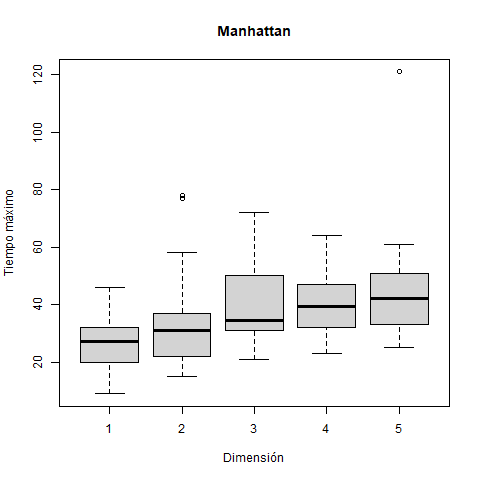
\includegraphics[width=70mm]{p1mr.png}
\caption   { Diagrama caja bigote.\label{Fig.1}
\label{p1mr.png}}
\end{figure}
\justify
Para un mayor entendimiento se determino el mínimo, promedio y máximo del tiempo de regreso por cada dimensión junto con el porcentaje de caminatas que nunca regresaron al origen los datos obtenidos se encuentran tabulados en el Cuadro \ref{tabla1}.
\begin{table}[h!]
    \caption{Indica el mínimo, promedio y máximo del tiempo de regreso por cada dimensión junto con el porcentaje de caminatas que nunca regresaron.}
    \label{tabla1}
    \centering
    \bigskip
    \begin{tabular}{||c||cr||cr||cr||cr|}
    Dimension & Mínimo &  Promedio & Máximo & Porcentaje\\
    1 & 2.0 &  8.5 & 10.0 & 37.5\% \\ 
    1 & 2.0 &  30.01 & 32.0 & 0\%  \\ 
    1 & 2.0 &  27.3 & 44.0 & 31.25\% \\ 
    1 & 2.000 &  18.9 & 74.000 & 42.1875\% \\
    1 & 2.000 &  25.03 & 116.000 & 54.6875\% \\
    1 & 2.0 &  45.02 & 256.0 & 50\% \\
    2 & 2.000 &  15.12 & 16.000 & 0\% \\
    2 & 2.000 &  8.3 & 8.000 & 75\% \\
    2 & 2.00 &  53.12 & 64.00 & 0\% \\
    2 & 2.00 &  59.135 & 118.00 & 7.8125\% \\
    2 & 2.000 &  17.3 & 30.000 & 88.28125\% \\
    2 & 2.0 &  51.15 & 66.0 & 87.109375\% \\
    3 & 2.000 &  6.365 & 10.000 & 37.5\% \\
    3 & 2.000 &  7.532 & 8.000 & 75\% \\
    3 & 2.00 &  39.78 & 42.00 & 34.375\% \\
    3 & 2.000 &  5.432 & 8.000 & 93.75\% \\
    3 & 2.00 &  60.465 & 68.00 & 73.4375\% \\
    3 & 2.0 &  72.03 & 82.0 & 83.984375\% \\
    4 & 2 &  58.3 & 6 & 62.5\% \\
    4 & 2.000 &  9.45 & 10.000 & 68.75\% \\
    4 & 2 &  2.35 & 2 & 96.875\% \\
    4 & 2.0 &  4.12 & 4.0 & 96.875\% \\
    4 & 2 &  12.16 & 10 & 96.09375\% \\
    4 & 2.0 &  31.19 & 32.0 & 93.75\% \\
    5 & 4 &  32.17 & 4 & 75\% \\
    5 & 2 &  17.8 & 2 & 93.75\% \\
    5 & 2.0 &  32.3 & 4.0 & 93.75\% \\
    5 & 2 &  64.17 & 8 & 89.76\% \\
    5 & 2.000 &  80 & 10.000 & 96.09375\% \\
    5 & 2 &  16 & 2 & 99.609375\% \\
    \end{tabular}
\end{table}

\newpage
\section{Conclusión}
\justify
Se demostró de manera sistemática los efectos de la dimensión en el tiempo de regreso al origen del movimiento de nuestra partícula o punto obteniendo como resultado que estas tardaran más en regresar al punto de origen o regresaran en una menor proporción a medida que la dimensión cambia.

\newpage
\section{Retos}

\justify
\textbf{Reto 1:} Estudiar de forma sistemática y automatizada el tiempo de ejecución de una caminata (en milisegundos) en términos del largo de la caminata (en pasos) y la dimensión. Para medir el tiempo de una réplica, ejecútala múltiples veces y normaliza con la cantidad de repeticiones para obtener un promedio del tiempo de una réplica individual.\cite{ejemplo}  %cita lo puesto en corchetes en la parte de referencias lo que esta en corchetes para citar se tiene que agregar en el apartado de un proyecto paralelo en este caso le puse el nombre ejemplo en el apartado de bibliografias para citar el ejemplo
\\
\\
\justify
\textbf{Reto 2:} Realizar una comparación entre una implementación paralela y otra versión que no aproveche paralelismo en términos del tiempo de ejecución, aplicando alguna prueba estadística adecuada para determinar si la diferencia es significativa.\cite{ejemplo}  %cita lo puesto en corchetes en la parte de referencias lo que esta en corchetes para citar se tiene que agregar en el apartado de un proyecto paralelo en este caso le puse el nombre ejemplo en el apartado de bibliografias para citar el ejemplo
%\\ Indica brincar espacio.

\clearpage
\bibliography{practica1} %\bibliography dentro de los corchetes aparece el comando seccion de referencias  sin embargo para que aparezca tiene que aparecer la seccion \bibliographystyle para dar un estilo del tipo de letra o tipo de acomodo que llevara 
\bibliographystyle{ieeetr}   %\da un estilo de acomodo dependiendo del comando dentro d corchetes
\end{document} %indica finalizacion de lo señalado en el parentesis en este caso el documento
